\chapter{Plantejament de l'hipòtesi}

Alhora de fer un experiment, podria haver anat per altres vies com la generació d'imatges amb color o la implementació d'una porta $X$ en una part específica del circuit quàntic que genera les imatges, que al posar-la o no, el model generes dos tipus d'imatges a través del mateix circuit. Tanmateix, les dues propostes requerien desenvolupar nous conceptes, ja que són idees pròpies. No em veia amb la confiança de poder implementar-les i obtenir objectius positius.

Llavors, al ser la implementació de les funcions no lineals un assumpte lleugerament conflictiu entre els diversos models de xarxes neuronals quàntiques, com ja he comentat en la secció \ref{qcircuits}.  Vaig decidir des d'un principi centrar-me en aquesta qüestió en concret.

La pregunta a investigar és la següent: \\
La incorporació d'una funció no lineal en el circuit quàntic generacional, a partir d'una mesura parcial, és la causa que el model arribi més ràpid al punt òptim?

En altres paraules, volia veure si la mesura parcial afectaria positivament en l'eficiència del model, fent que la generació de les imatges desitjades es donés a terme en un menor temps.

Sembla una qüestió senzilla, però la dificultat de l'experiment radica en crear la xarxa neuronal en si, amb totes les seves parts accessibles per poder fer els canvis que siguin necessaris. L'única manera de fer l'experiment seria programant el model, una tasca que tenia clar que faria des del principi.

\chapter{Programació del model}

Posteriorment a començar a programar el model, ja tenia clar que ho havia de fer en \textit{Python}. En el passat creat alguns algoritmes i tenia experiència construint i executant circuits quàntics amb \textit{Cirq} \cite{cirq}, una eina desenvolupada per Google. A més a més, sabia de l'existència de \textit{TensorFlow Quantum} \cite{tfq}, una altra eina desenvolupada per Google destinada a la creació de xarxes neuronals quàntiques i algoritmes de \textit{quantum mechine learning} en general. També tenia una mica d'experiència en aquest \textit{framework}. Per tant, desenvolupar el model en \textit{TensorFlow Quantum} va ser la primera opció. 

Tenia pensat basar el meu codi en el tutorial de \textit{TensorFlow} sobre una xarxa convolucional generativa adversària. Havia de canviar el generador per un circuit quàntic que s'optimitza a partir d'un diferenciador\footnote{Objecte que calcula el gradient d'un circuit quàntic.} automàtic provinent de \textit{TensorFlow Quantum} \cite{tfq}. 

També havia de canviar l'arquitectura del discriminador. Havia de ser una xarxa més simple amb unes poques capes totalment connectades.

El primer problema que em vaig trobar va ser la creació del \textit{dataset} que alimenta a la xarxa discriminativa. A causa de la peculiaritat de les imatges que volia generar, havia de crear-lo manualment. Usualment les imatges que componen els \textit{datasets} utilitzats en \textit{deep machine learning} són extretes de bancs d'informació amb mides enormes. En el meu cas, havien de ser generades per mi, per tant havia de convertir matrius de \textit{Numpy} en \textit{datasets} de \textit{TensorFlow}. Recordo que en va costar arribar a tindre la solució a aquest problema. 

\section{Discriminador}

Una vegada ja tenia fet el \textit{dataset} em vaig posar a fer el model. En el tutorial per una \href{https://www.tensorflow.org/tutorials/generative/dcgan}{DCGAN (GAN convolucional)} els dos models eren entrenats per la funció \code{train\_step()}, que representa una iteració en el procés d'optimització. En aquesta es crida a la funció \code{tf.GradientTape} per guardar el diferenciador automàtic. El problema que vaig dintre amb aquesta funció és que directament no funcionava amb el discriminador, aquest no era optimitzat. Després d'intentar solucionar l'error pels meus propis medis, mirant la causa d'aquest i de buscar a fòrums la solució o causa, em vaig rendir. Ja havia estat uns quants mesos intentant desenvolupant el model amb \textit{TensorFlow} i \textit{TensorFlow Quantum}. Havia creat les capes del generador quàntic manualment, també ho havia fet amb l'optimitzador\footnote{No sabia ni si funcionarien adequadament, pel fet que per provar-ho, havia de tenir tot el model enllestit.}. Tenia el model gairebé acabat, però perquè no podia optimitzar el discriminador em vaig veure obligat a canviar d'estratègia.

Existeixen dos grans \textit{frameworks} per crear i executar circuits quàntics: \textit{Cirq} \cite{cirq}, desenvolupat per Google, i \textit{Qiskit} \cite{qiskit}, creat per IBM. Una vegada vaig decidir no continuar amb \textit{Cirq}, havia de provar amb \textit{Qiskit}. La veritat, havia d'haver començat amb \textit{Qiskit} des del principi, és més útil (té moltes més característiques), i el més important, té una major comunitat, per tant, és més fàcil trobar solucions a l'error que pots tenir i és més fàcil trobar a persones disposades a ajudar-te.

Igual que \textit{Cirq} té un \textit{framework} per poder desenvolupar xarxes neuronals (\textit{TensorFlow Quantum}); \textit{Qiskit} també té el seu, anomenat \textit{PyTorch} \cite{pytorch_2019}, no obstant no té una integració tan directa, ja que no estan desenvolupats pel mateix equip, ni la mateixa companyia.

Per tant, en canviar de \textit{Cirq} a \textit{Qiskit}, també havia de canviar de \textit{TensorFlow} a \textit{PyTorch}, però no tenia res d'experiencia amb PyTorch, sabia que la transició seria complicada, i tenia raó. No vaig ni aconseguir crear el \textit{dataset} d'imatges per alimentar al discriminador.

Després d'intentar-lo amb \textit{TensorFlow Quantum} i amb \textit{PyTorch}, vaig decidir prescindir de \textit{frameworks} per crear models de \textit{machine learning}. Crearia tant el discriminador com el generador manualment. 

El discriminador, al ser una xarxa tan simple, la podria crear des de zero. Llavors vaig començar a buscar codi a internet que pogués utilitzar. Volia una xarxa neuronal feta amb \textit{Numpy}, una llibreria de \textit{Python} per fer càlculs amb vectors i matrius amb la qual tenia bastant experiència.

Després de provar dues opcions que més o menys m'agradaven\footnote{Buscava codi estructurat d'una forma en concret, que estigui dissenyat amb la filosofia de \textit{Object Oriented Programming}, una forma d'escriure codi en el qual tot s'implementa en un sol objecte.}, va aparèixer un repositori\footnote{\href{https://github.com/mnielsen/neural-networks-and-deep-learning}{Enllaç del respositori de Michael Nielsen}, la persona que més m'ha ajudat a fer aquest treball. Però no m'ha ajudat directament, ho dic perquè és el coautor de \textit{QC i QI} \cite{QCandQI} i autor de la xarxa neuronal que va fer que progressés amb la programació. } de Michael Nielsen, coautor de \textit{Quantum Computation and Quantum Information} \cite{QCandQI} que em va salvar. 

El repositori tenia codi per xarxes neuronals que estava estructurat d'una forma que m'agradava i encara més important, que entenia. Inclús tènia diverses versions d'una mateixa xarxa neuronal, amb un nivell de complexitat diferent. Llavors, a partir del model més simple que hi havia en el repositori \footnote{Es pot veure el codi original a l'annex \ref{lst:disc_original}.}, vaig començar a desenvolupar el discriminador.

Per verificar el correcte funcionament del discriminador, i per poder comprendre com funciona el codi, vaig utilitzar la teoria del capítol \ref{ML}. No obstant això, el principal problema que em vaig trobar va ser derivar la funció de pèrdua, per exemple la \textit{Minimax}, s'ha de derivar-la a partir de dues equacions, una per a cada etiqueta.

Com es pot veure al codi final pel discriminador a l'annex \ref{lst:disc_final}, he fet bastants canvis, però no he canviat l'estructura del codi. La majoria dels canvis són per afegir més funcionalitat al model, com per exemple l'emmagatzematge de les dades per poder al final veure-les en un gràfic. Tanmateix, si que vaig haver-hi de canviar la funció de pèrdua utilitzada, ja que originalment, era una MSE.

El canvi més important és que inclou les dues formes d'optimitzar el model, amb dues funcions de pèrdua que funcionen de manera diferent, però que són la mateixa, la \textit{Binary Cross Entropy} i la \textit{Minimax}. Això en el codi està materialitzat en dues funcions\footnote{Funcions de \textit{Python}.} diferents, \code{backprop\_bce()} i \code{backprop\_minimax()}. No tenen cap diferència en termes d'eficàcia o rapidesa i les vaig fer tan sols per comprovar aquest fet. 

Mirant enrere, és una tasca fàcil, però en el moment vaig tindre moltes dificultats alhora d'adaptar el codi a les meves necessitats. Un aspecte que em va ajudar molt va ser comprendre la teoria darrera de les xarxes neuronals que he presentat a la secció \ref{gradient_descent}.

El codi final del discriminador es pot veure a l'annex \ref{lst:disc_final}. També en el repositori d'aquest treball hi ha un altre arxiu que conté una altra versió en la qual intentava implementar diverses funcions d'activació en el model, però no ho vaig aconseguir, tanmateix, no em preocupa perquè no és una part vital del treball, no passa res per tindre el discriminador només amb la funció sigmoide com a funció d'activació. Tenia l'intenció de fer-ho perquè en l'article de Huang et. al., la funció d'activació que s'utilitza és la \textit{ReLu} \cite{QGAN_exp}. 

\section{Generador}

El desenvolupament de l'altra part del model, el generador, va ser molt diferent. Després de provar de fer-ho amb \textit{TensorFlow Quantum}, sense obtenir bons resultats, no tenia altra opció que fer-ho tot manualment i jo mateix\footnote{No em vaig ni plantejar buscar codi per internet perquè pensava que els autors dels papers que vaig llegir, les úniques persones que sabia que podien tindre el codi, no el penjarien.}, això no obstant, ja tenia experiència en fer petites xarxes neuronals quàntiques i això em tranquil·litzava. Sabia perfectament el que havia de fer, i com ho havia de fer: Implementar el mètode de \textit{parameter shift} en els circuits quàntics dels quals he parlar en la secció \ref{qcircuits}.

Una vegada tenia la funció que creava els circuits quàntics, em vaig posar amb l'optimització dels paràmetres, de la qual parlaré a continuació.

Primer de tot cal remarcar que el model s'optimitza a partir d'un \textit{batch}, és a dir, un grup de dades, en aquest cas, un grup d'imatges. S'agafa la mitjana dels errors de cada \textit{batch}, i s'actualitzen els paràmetres a partir d'aquesta. La motivació per treball en \textit{batch} i no dades individuals és perquè s'ha de mirar l'error d'unes quantes dades a la vegada, d'aquesta manera l'optimització és més robusta \cite{GAN2014}.

Tornant al funcionament de l¡optimització, ho explicaré tal i com està implementat en el codi. Per començar s'han d'agafar els paràmetres a optimitzar, que estaran en forma d'un vector $\theta$, escollir un d'ells que anomenaré $\theta_{i}\,$, que és el paràmetre que s'optimitzarà, i crear un vector de pertubació $\Delta_{i}\,$. 

Llavors es creen dos vectors de paràmetres nous, $\theta^{+}_{i}$ i $\theta^{+}_{i}$: Es multiplica $\pm\frac{\pi}{4}$ pel vector de pertubació, i es suma el resultat al vector de paràmetres original\footnote{Cada un d'aquests vectors de paràmetres té una petita variació en un paràmetre, i cada vector té una variació en un sentit.}. 

A continuació, es creen dues imatges, cadascuna corresponent a un dels vectors de paràmetres creats, una amb $\theta^{+}_{i}$ i l'altra amb $\theta^{-}_{i}\,$. 

Per últim, s'avalua la funció de pèrdua per a cada imatge generada i es treu la diferència entre elles, d'aquesta manera calculant una derivada $\pdv{\mathcal{L}}{\theta_i}$ respecte al paràmetre $\theta_{i}\,$.

Una vegada es té una derivada per a cada paràmetre de $\theta$ es pot construir el vector gradient $\nabla_\theta$. He de dir que aquest vector té la mateixa mida que el vector $\theta\,$, com que cada element en el gradient correspon a la derivada d'un paràmetre de $\theta$.

Al llarg de l'optimització es van sumant les derivades a $\nabla_\theta$, si això es fa per a tots els paràmetres de $\theta$ i per a totes les dades del \textit{batch}, finalment es pot treure la derivada mitjana dividint els elements de $\nabla_{\theta}$ per la quantitat de dades que hi ha en un \textit{batch}.

Amb el gradient $\nabla_{\theta}$ es poden finalment optimitzar tots els paràmetres, d'acord amb les derivades (concretament la mitjana de moltes derivades) de les quals està compost. 
 
 
\begin{figure}
	\HRule \\
	\textbf{Algorithm 2 Pseudocodi per una xarxa generativa adversària quàntica} \\
	\HRule \\
	\begin{algorithmic}
		\State{$\nabla = 0$} \Comment{Creació del vector  $\nabla$ que té la mateixa mida que $\theta$}
		\For{soroll en batch}
		\For{paràmetre $\theta_i$ en  $\theta$}
		\State{$\Delta_i = 0$} \Comment{Creació del vector pertubació d'acord amb el vector $\theta$}
		\State{$\theta^{+}_i = \theta + \frac{\pi}{4}\Delta_i$}
		\State{$\theta^{-}_i = \theta - \frac{\pi}{4}\Delta_i$}
		\\
		\State{Imatge\textsubscript{1} = generador(soroll, $\theta^+_i$) } 
		\State{Imatge\textsubscript{2} = generador(soroll, $\theta^-_i$) } \Comment{Generació de les imatges}
		\\
		\State{Predicció\textsubscript{1} = discriminador(Imatge\textsubscript{1})} 	\State{Predicció\textsubscript{2} = discriminador(Imatge\textsubscript{2})} \Comment{El discriminador posa una etiqueta a cada imatge}
		\\
		\State{Diferencia\textsubscript{$i$} = $\mathcal{L}$(Predicció\textsubscript{1}) - $\mathcal{L}$(Predicció\textsubscript{2})}
		\\
		\State{$\nabla_\theta = \nabla_i + $ Diferencia\textsubscript{$i$}} \Comment{On $\mathcal{L}$ és la funció de pèrdua del generador}
		\EndFor
		\EndFor
		\\
		\For{$\theta_i$ en $\theta$ i $\nabla_i$ en $\nabla_\theta$} \Comment{Per a cada paràmetre i per a cada error}
		\State{$\theta^{t+1}_i = \theta_i + \frac{\eta}{M}\nabla_i$} \Comment{Actualització del paràmetre amb la mitjana de l'error que correspon a aquest paràmetre}
		\EndFor
	\end{algorithmic}
	\HRule \\[-.4cm]
	\caption{ Em refereixo a l'input de la xarxa generacional com a soroll, ja que és més encertat d'aquesta manera. El vector $\nabla$ té la mateixa mida que el vector de paràmetres $\theta$, cal notar que també té la mateixa mida els vectors $\theta^\pm_i$, ja que aquests vectors són $\theta$ amb una alteració al paràmetre $\theta_i$. Les paraules \textit{generador} i \textit{discriminador} denoten els respectius models, per tant, \textit{Imatge\textsubscript{$i$}} i \textit{Predicció\textsubscript{$i$}} són els outputs dels models.}
	\label{fig:alg_gen}
\end{figure}

El pseudocodi per aquest procediment es pot trobar en la figura \ref{fig:alg_gen}. En aquesta es pot veure que es crida al discriminador perquè posi etiquetes a les dues imatges generades, això és per poder avaluar aquestes etiquetes amb la funció de pèrdua. Per després poder agafar la diferència i d'aquesta manera calcular la derivada. El codi pel generador es pot trobar en l'annex, \ref{lst:gen_final}.

\section{Creació del model}

Quan ja es tenen les dues parts del model, aquestes s'han d'ajuntar d'alguna manera. El que jo he fet és posar-ho tot en una classe de \textit{Python} anomenada \code{Quantum\_GAN}, que conté les funcions per definir el model, per executar-lo, per guardar les seves dades i per crear els gràfics que serveixen per avaluar l'eficiència del model. Aquesta classe és el tros de codi que junta tot, tant el discriminador i el generador. També agafa altres funcions que són necessàries, com per exemple la sigmoide. Aquestes funcions que no estan en l'arxiu del generador ni en el del discriminador, es troben en \code{functions.py}.

S'han de tenir en compte algunes de les funcionalitats d'aquesta classe. En particular, com circulen les dades del generador als discriminadors i com es creen les gràfiques amb les quals valoro l'eficiència dels models.

La funció que s'utilitza per entrenar el model és \code{Quantum\_GAN.train()}. Aquesta té com input un \textit{dataset} amb imatges reals i el soroll per poder entrenar el generador. Aquest \textit{dataset} es divideix en grups d'imatges (els \textit{batchs}), cada \textit{batch} conté tant imatges reals, com soroll en la mateixa quantitat.

En una iteració primer s'optimitza el generador, que substitueix el soroll del \textit{batch} amb les imatges que genera. Llavors es passa el \textit{batch} al discriminador que s'optimitza tant amb les imatges reals com amb les imatges falses. Aquest és el procés pel qual s'optimitzen els dos models. 

Pel que fa a la creació de les gràfiques, aquesta classe selecciona una imatge real aleatòria i una de falsa per avaluar la funció de pèrdua en la iteració, també crea les etiquetes utilitzades en aquesta l'avaluació. Totes aquestes dades s'utilitzen per a la creació de diversos gràfics que mostren l'evolució d'aquestes dades a través de tota l'optimització.

\section{Execució del model}

No obstant això, en l'arxiu \code{qgan.py}, no es troba l'execució del model, només està la definició de la classe \code{Quantum\_GAN}. Això és perquè el codi realment s'executa en l'arxiu \code{main.py}. Aquest és l'únic arxiu que té codi que realment s'executa, els altres arxius només tenen definicions. Per projectes relativament grans, com aquest, convé tenir un arxiu que fa tot el treball, el qual crida a totes les funcions definides en altres arxius i les executa d'una manera ordenada. 

Com es pot veure en l'annex, \ref{lst:main}, aquest arxiu té molt poc codi. En ell només es crea amb \textit{Numpy} el dataset, es defineix el discriminador i el generador, amb els quals es crea el model amb \code{Quantum\_GAN}. 

Finalment, es crida a la funció \code{Quantum\_GAN.train()} per optimitzar el model. En acabar l'optimització es criden les funcions \code{Quantum\_GAN.plot()}, \code{Quantum\_GAN.create\_gif()} i \code{Quantum\_GAN.save()}, les quals donen a terme funcions complementàries com la creació de les gràfiques, la creació d'un GIF que mostra com les imatges vam evolucionar al llarg de l'optimització, i l'emmagatzematge de les dades rellevants que s'han creat durant l'optimització.

Les imatges que vaig escollir per generar són les mateixes que van generar en l'article en el qual vaig basar el treball. No entraré molt en detall sobre les distribucions concretes que formen les imatges, però per tindre una imatge general sobre com són es pot veure la figura \ref{fig:test_images}. O directament es pot consultar les distribucions en l'article original \cite{QGAN_exp} o veure com es generen les imatges en el codi \ref{lst:main}. 

\begin{figure}
	\begin{subfigure}{0.5\textwidth}
		\begin{centering}
			
\includegraphics[width=0.65\linewidth]{Figures/test_images}
			\caption{}
			\label{fig:fake_image}
		\end{centering}
	\end{subfigure}
	\begin{subfigure}{0.5\textwidth}
		\begin{centering}
			
\includegraphics[width=0.65\linewidth]{Figures/fake_image}
			\caption{} 
			\label{fig:real_image}
		\end{centering}
	\end{subfigure}
	\caption{\textbf{A)} Aquest és un exemple d'una imatge del \textit{dataset} amb el qual s'entrena el model que he creat. És simplement una imatge en blanc i negre de 4 píxels, en la qual hi ha dos píxels amb un valor aproximant de $0.5$ i els altres dos amb un valor de $0$. Les imatges es creen a partir d'una \textit{array} de \textit{Numpy}, com per exemple \code{np.array([[0.47804505, 0.], [0.47804505, 0.]])}. \textbf{B)} Aquest és un exemple d'una imatge generada que tracta de ser el més semblant possible a les imatges del \textit{dataset}. Es pot veure que són indistingibles a simple vista, però al veure els valors es pot apreciar com els nombres no són els mateixos: \code{np.array([[0.504324, 0], [0.495676, 0]])} . Això és perquè només pel valor de $0.5$ és possible tenir els dos píxels amb el mateix valor, sempre que els valors dels altres píxels sigui zero. Cal recordar que els valors dels píxels han de sumar $1$. Ja que són valors generats per un circuit quàntic. Per tant, les imatges del \textit{dataset} com la que he mostrat no són possibles de crear. He pensat fer-ho d'aquesta manera per veure si es generaria les imatges correctament amb aquesta limitació, el resultat ha sigut que les imatges que es generen són com la mitjana dels valors de les imatges del \textit{dataset}, tal com es pot apreciar en la figura \ref{fig:700_images}. }
	\label{fig:test_images}
\end{figure}


Si executen el model, amb una mida de \textit{batch} de $10$, tant el \textit{learning rate} del discriminador com del generador a $0.1$, i un total d'iteracions de $400$, hi ha una garantia d'arribar a la convergència desitjada, és dir que, que els dos models arriben a l'equilibri de Nash i no poden continuar l'optimització. En aquest punt és quan les imatges falses i les reals són iguals.
\begin{figure}[H]
	\label{fig:labels_loss_400}
	\begin{subfigure}{0.5\textwidth}
		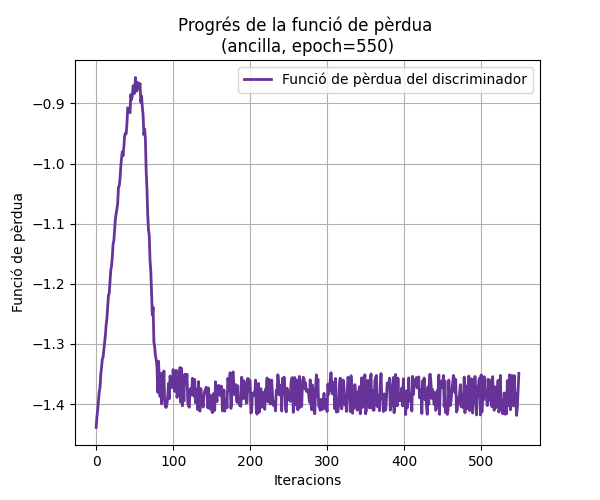
\includegraphics[width=\linewidth]{figures/model/loss_plot.png}
		\caption{}
		\label{fig:loss_400}
	\end{subfigure}
	\begin{subfigure}{0.5\textwidth}
		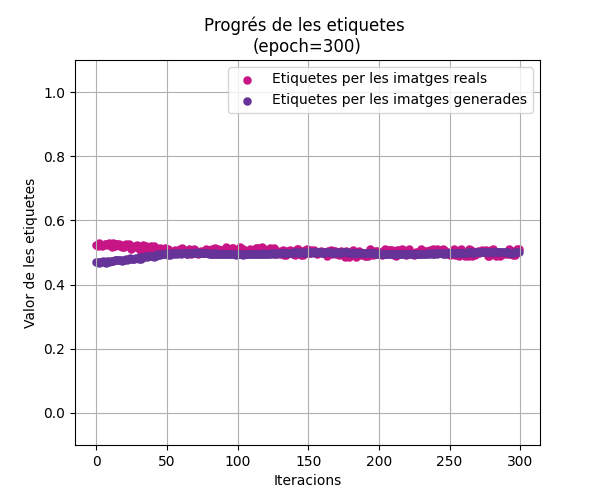
\includegraphics[width=\linewidth]{figures/model/labels_plot.png}
		\caption{} \label{fig:labels_400}
	\end{subfigure}
	\caption{En aquestes figures es pot veure com per la iteració 250, el model ja s'ha estabilitzat. Això és perquè les etiquetes i el valor de la funció de pèrdua convergeixen en un valor. \textbf{A)} Funció de pèrdua per cada iteració. A partir de la iteració 175, es pot veure com el valor de la funció s'estabilitza en l'interval $(-1.35, -1.4)$, això concorda amb els valors de les etiquetes en les mateixes iteracions, ja que $\log(\frac{1}{2}) + \log(1-\frac{1}{2}) \simeq -1.38$. \textbf{B)} Etiquetes per les imatges reals i generades per cada iteració. Es pot observar que els valors de les etiquetes per les imatges reals són més inestables que els valors de les generades. Això és perquè les imatges reals tenen una major variació en els valors dels píxels, mentre que en les generades aquest fet no és tan notable. Per tant, el discriminador assigna etiquetes amb una major variació.}
\end{figure}

En la figura, \ref{fig:labels_400}, es pot veure com les etiquetes pels dos tipus d'imatges van oscil·lant fins a estabilitzar-se. El mateix es pot dir per la funció de pèrdua, com es pot veure en la figura \ref{fig:loss_400}.  

A causa del fet que aquests gràfics són molt semblants als seus anàlegs de les GANs clàssiques i que les distribucions reals i generades són pràcticament iguals (com es pot veure a la figura \ref{fig:comp_imatge}), considero que el model funciona correctament.


\begin{figure}[H]
	\begin{subfigure}{0.51\textwidth}
		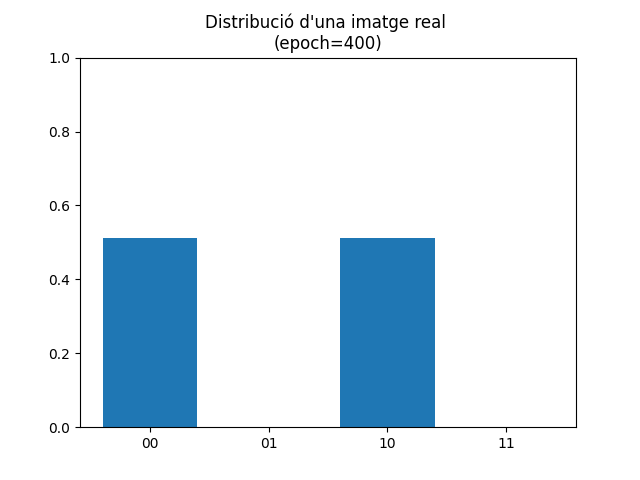
\includegraphics[width=\linewidth]{figures/model/real_distribution.png}
		\caption{Distribució d'una imatge real} \label{fig:1a}
	\end{subfigure}%
	\hspace*{\fill}   % maximize separation between the subfigures
	\begin{subfigure}{0.51\textwidth}
		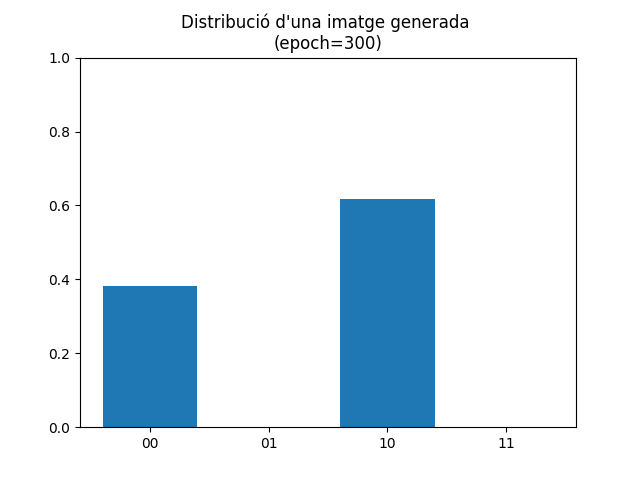
\includegraphics[width=\linewidth]{figures/model/fake_distribution.png}
		\caption{Distribució d'una imatge generada} \label{fig:1b}
	\end{subfigure}%
	\hspace*{\fill}
	\caption{Comparació d'una imatge generada i una real, quan el model ha assolit la convergència. En l'eix Y es pot veure el valor d'un píxel, mentre que en l'eix X estan els píxels. }
	\label{fig:comp_imatge} 
\end{figure}


Abans he especificat que al cap de $400$ iteracions podem tenir la garantia d'arribar al punt d'equilibri, no obstant això, es pot arribar a aquest punt amb menys iteracions, el que vull dir és que amb $400$ de segur que s'arriba. Això és perquè, com a tots els models de \textit{machine learning} hi ha una part de sort implicada. Si els paràmetres inicials són més semblants als paràmetres desitjats, el model assolirà la convergència més ràpidament.
 
\chapter{Realització del experiment} 

Una vegada havia confirmat el correcte funcionament del model, vaig començar amb el desenvolupament del experiment. Havia de crear els dos tipus de circuits quàntics que necessitava, uns amb un sistema ancilla, i uns altres sense.

Un sistema ancilla, és un grup de qubits sobre els quals es donen a terme operacions, però que no es mesuren per treure l'output del circuit. Aquests qubits es pot veure clarament en la figura \ref{fig:qcircuit}. 

\begin{figure}
	\begin{quantikz}
		\lstick[wires=2]{$\mathcal{A}$}& & \lstick{$\ket{0}$} &  \gate{I}& \gate{U_{\theta_{1, l}}} & \ctrl{1} & \qw & \qw & \qw & \gate{U_{\theta_{1, l-1}}} & \ctrl{1} & \qw & \qw & \qw & \qw  \\
		& & \lstick{$\ket{0}$} &  \gate{I} & \gate{U_{\theta_{2, l}}} & \control{} & \ctrl{1} & \qw & \qw & \gate{U_{\theta_{2, l-1}}} & \control{} & \ctrl{1} & \qw & \qw & \qw  \\
		&&\lstick{$\ket{0}$} &  \gate{R_y(\alpha_3)} & \gate{U_{\theta_{3, l}}} & \qw & \control{} & \ctrl{1} & \qw & \gate{U_{\theta_{3, l-1}}} & \qw & \control{} & \ctrl{1} & \qw &  \meter{} \\
		&&\lstick{$\ket{0}$} &  \gate{R_y(\alpha_4)} & \gate{U_{\theta_{4, l}}} & \qw & \qw & \control{} & \ctrl{1} & \gate{U_{\theta_{4, l-1}}} & \qw & \qw & \control{} & \ctrl{1} &  \meter{} \\
		&&\lstick{$\ket{0}$} &  \gate{R_y(\alpha_5)} & \gate{U_{\theta_{5, l}}} & \qw & \qw & \qw & \control{} & \gate{U_{\theta_{5, l-1}}} & \qw & \qw & \qw & \control{}  & \meter{}
	\end{quantikz}
	\caption{Aquí he marcat els qubits ancilla amb $\mathcal{A}$, són els dos primers. També al final del circuit he afegit mesures als qubits que s'han de mesurar.}
	\label{fig:qcircuit}
\end{figure}

Primer de tot he de mencionar que havia de fer alguns canvis al generador per acomodar aquests qubits ancilla. 

Segon, cal notar que no he replicat exactament la metodologia emprada en l'article original. En ell tenen aquesta equació \cite{QGAN_exp}: 
\begin{equation*}
\rho = \frac{\tr_A(\Pi_A \ket{\psi}\bra{\psi})}{\tr(\Pi_A\otimes I_{2^N-2^{N_A}}\ket{\psi}\bra{\psi})}
\end{equation*}

Com ja he comentat en la secció \ref{par_measurament}, no veig com aquesta equació pot tenir sentit, per tant la vaig ometre del meu experiment. 

L'alternativa que he fet servir són els mesuraments de \textit{Qiskit}, al definir el circuit especifico quins són els qubits que no vull mesurar, que són els qubits que formen part del sistema ancilla. No obstant això, no sé exactament quin és el funcionament d'aquest mètode. Però si empro aquest procediment en altres circuits, dels quals sé el resultat, aquest mètode fa el que m'espero\footnote{Parlo dels parells de Bell, els circuits quàntics amb entrellaçament més simples que es poden fer.}.

L'arxiu que utilitzo per fer els experiments és \code{experiment.py}. En ell es pot veure com defineixo dos discriminadors\footnote{Que tenen les mateixes característiques.} i dos generadors, que es diferencien pels circuits que fan servir, un amb qubits ancilla i l'altre sense. Aquests models s'agrupen en parelles per definir dues qGANs.

Cal notar que els generadors i els discriminadors\footnote{Al principi pensava no tenir els mateixos paràmetres inicials pels discriminadors, però al veure les gràfiques de les etiquetes, l'efecte que tenen aquests és molt notable. Es pot veure com a vegades les etiquetes comencen en uns valors de $1$ i en altres de $0$. \href{https://drive.google.com/file/d/1kYZ1vmNYU17sofNluXFYnoATLfY5B0jG/view?usp=sharing}{enllaç per veure una imatge amb totes les gràfiques} (perdó per la informalitat)} comencen amb els mateixos paràmetres, per tant, tenen les mateixes condicions, menys els circuits quàntics és clar. També s'utilitza el mateix \text{dataset}.

\section{Anàlisi dels resultats}
Si comparem les gràfiques que mostren les etiquetes es pot veure una clara diferencia: Els models que tenen els circuits amb els qubits ancilla són més inestables que el que no els tenen, tal i com es pot veure en la figura \ref{fig:700_labels}. Tanmateix, això no vol dir necessàriament que siguin més eficients. 

També es pot observar una clara diferència en les imatges generades en la primera iteració. En les primeres imatges d'un generador amb la funció no lineal es pot veure un píxel amb un valor de $1$ mentre que els altres estan al $0$. Mentre que en l'altre tipus de generador es pot veure que els píxels tenen més o menys el mateix valor, d'aquesta manera formant una distribució uniforme. 

Aquest fet probablement és causat per l'estructura del circuit que té els qubits ancilla. Tanmateix, perquè exactament passa això està fora dels meus coneixements sobre la matèria\footnote{Saber com es comporten sistemes quàntics que tenen parts entrellaçades.}.

\begin{figure}[H]
	\begin{subfigure}[b]{.32\linewidth}
		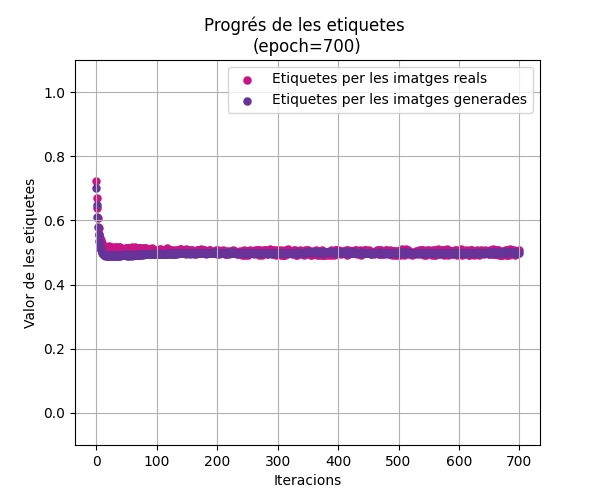
\includegraphics[width=\linewidth]{figures/data/L_4.png}
		\caption{}
	\end{subfigure}
	\begin{subfigure}[b]{.32\linewidth}
		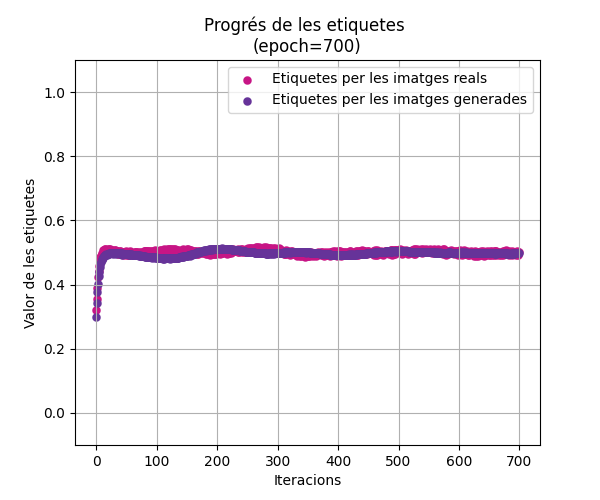
\includegraphics[width=\linewidth]{figures/data/L_5.png}
		\caption{}
	\end{subfigure}
	\begin{subfigure}[b]{.32\linewidth}
		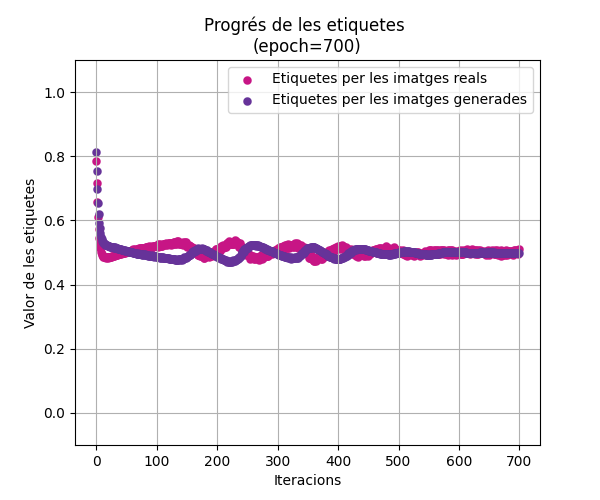
\includegraphics[width=\linewidth]{figures/data/L_6.png}
		\caption{}
	\end{subfigure}
	
	\begin{subfigure}[b]{.32\linewidth}
		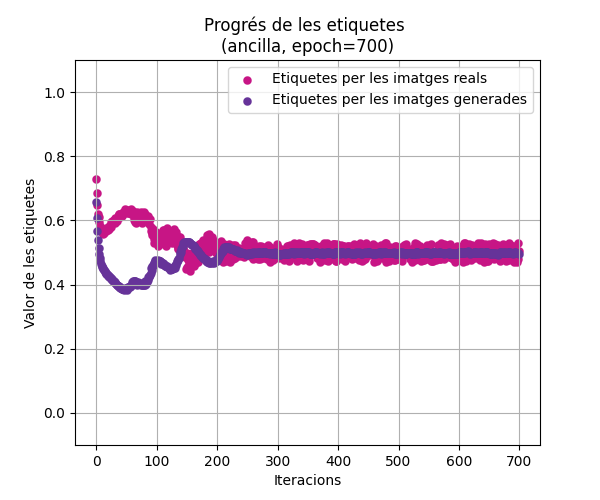
\includegraphics[width=\linewidth]{figures/data/L_A4.png}
		\caption{}
	\end{subfigure}
	\begin{subfigure}[b]{.32\linewidth}
		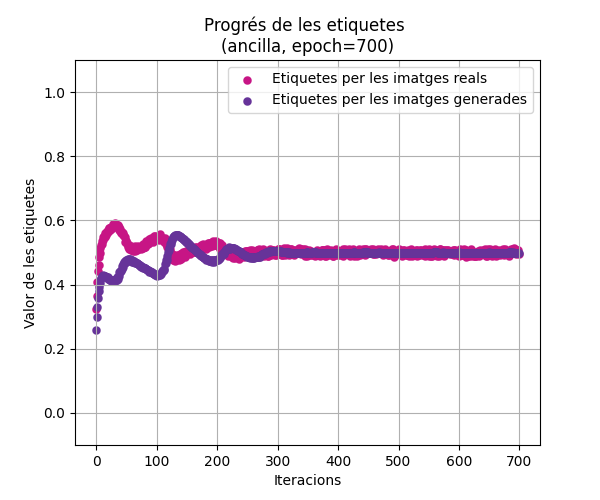
\includegraphics[width=\linewidth]{figures/data/L_A5.png}
		\caption{}
	\end{subfigure}
	\begin{subfigure}[b]{.32\linewidth}
		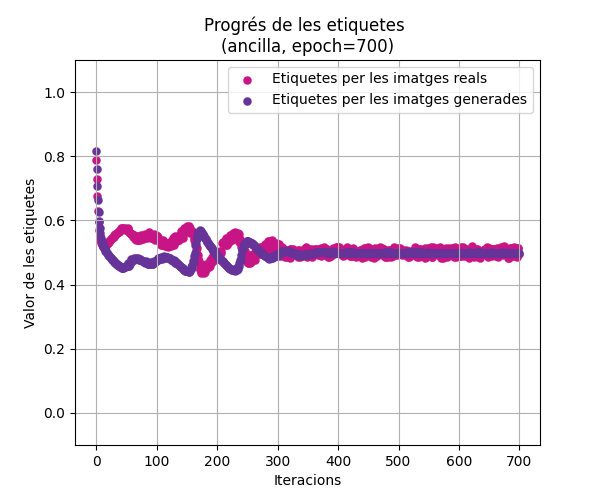
\includegraphics[width=\linewidth]{figures/data/L_A6.png}
		\caption{}
	\end{subfigure}
	\caption{Es pot apreciar com els models sense la funció no lineal (\textbf{A}, \textbf{C}, \textbf{B}) tenen una major estabilitat en les etiquetes comparats amb els models que sí tenen la funció no lineal (\textbf{D}, \textbf{E} i \textbf{F}).}
	\label{fig:700_labels}
\end{figure}

La part que realment m'intriga és que durant les primeres iteracions, en els circuits amb els qubits ancilla el píxel que té el valor de $1$, passa d'un a un altre. Aquest comportament succeeix  cada vegada que he executat el codi. Igual que he dit abans, arribar a comprendre la causa d'aquest fet està fora de les meves capacitats.

Estic bastant segur que aquesta fluctuació dels píxels és el factor que causa la inestabilitat que es pot observar en les etiquetes.

Després de mirar les gràfiques que generaven els models, vaig posar-me a redactar les conclusions, malgrat això, no estava satisfet amb la precisió de l'anàlisi de les dades. No podia saber amb certesa quin dels dos tipus de models era el més eficient. 

Necessitava una mètrica que en digués quina és la semblança entre les imatges generades i les imatges reals. Sabia que en l'article en el qual he basat el treball els autors havien fet servir una mètrica anomenada \textit{Férchet Score} o puntuació de Férchet \cite{QGAN_exp}, en la qual s'emprava la distància de Férchet. Aquesta distància serveix per comparar dues distribucions a partir de la seva mitjana i la seva covariància \cite{sd_score}.

Llavors vaig decidir implantar aquesta mètrica, i veure com evoluciona al llarg de l'optimització. 

En un article sobre l'avaluació de les imatges generades per les GAN \cite{sd_score}, vaig trobar aquesta equació per calcular la distància de Férchet:
$$
FD(r, g) = \abs{\mu_r - \mu_g}^2 + \tr(\Sigma_r + \Sigma_g -2(\Sigma_r\Sigma_g)^{\frac{1}{2}})
$$

On $\mu$ és la mitjana\footnote{He emprat la mitjana aritmètica.} i $\Sigma$ és la covariància d'una distribució. Aquesta equació l'he implementat en \textit{Python} mitjançant matrius, és a dir les imatges. La covariància és calculada amb una funció de \textit{Numpy}. A la qual se li dona com input una matriu on cada fila d'aquesta representa una variable d'una distribució. No puc estar 100\% segur de què he implementat aquesta mètrica correctament, ja que no sé el funcionament exacte de la covariància, ni el de la funció de \textit{Numpy}. No obstant això, sembla que funciona correctament.

Cal notar que si les dues imatges són exactament iguals, la distancia dona pràcticament zero\footnote{Python diu que és d'un ordre de magnitud de $10^{-16}$ aproximadament.}. Per considerar que dues imatges són «acceptablement semblants», han de tenir una distància entre elles de $10^{-3}$ aproximadament.